\section{Auswertung}
\label{sec:Auswertung}

\begin{figure}[H]
  \centering
  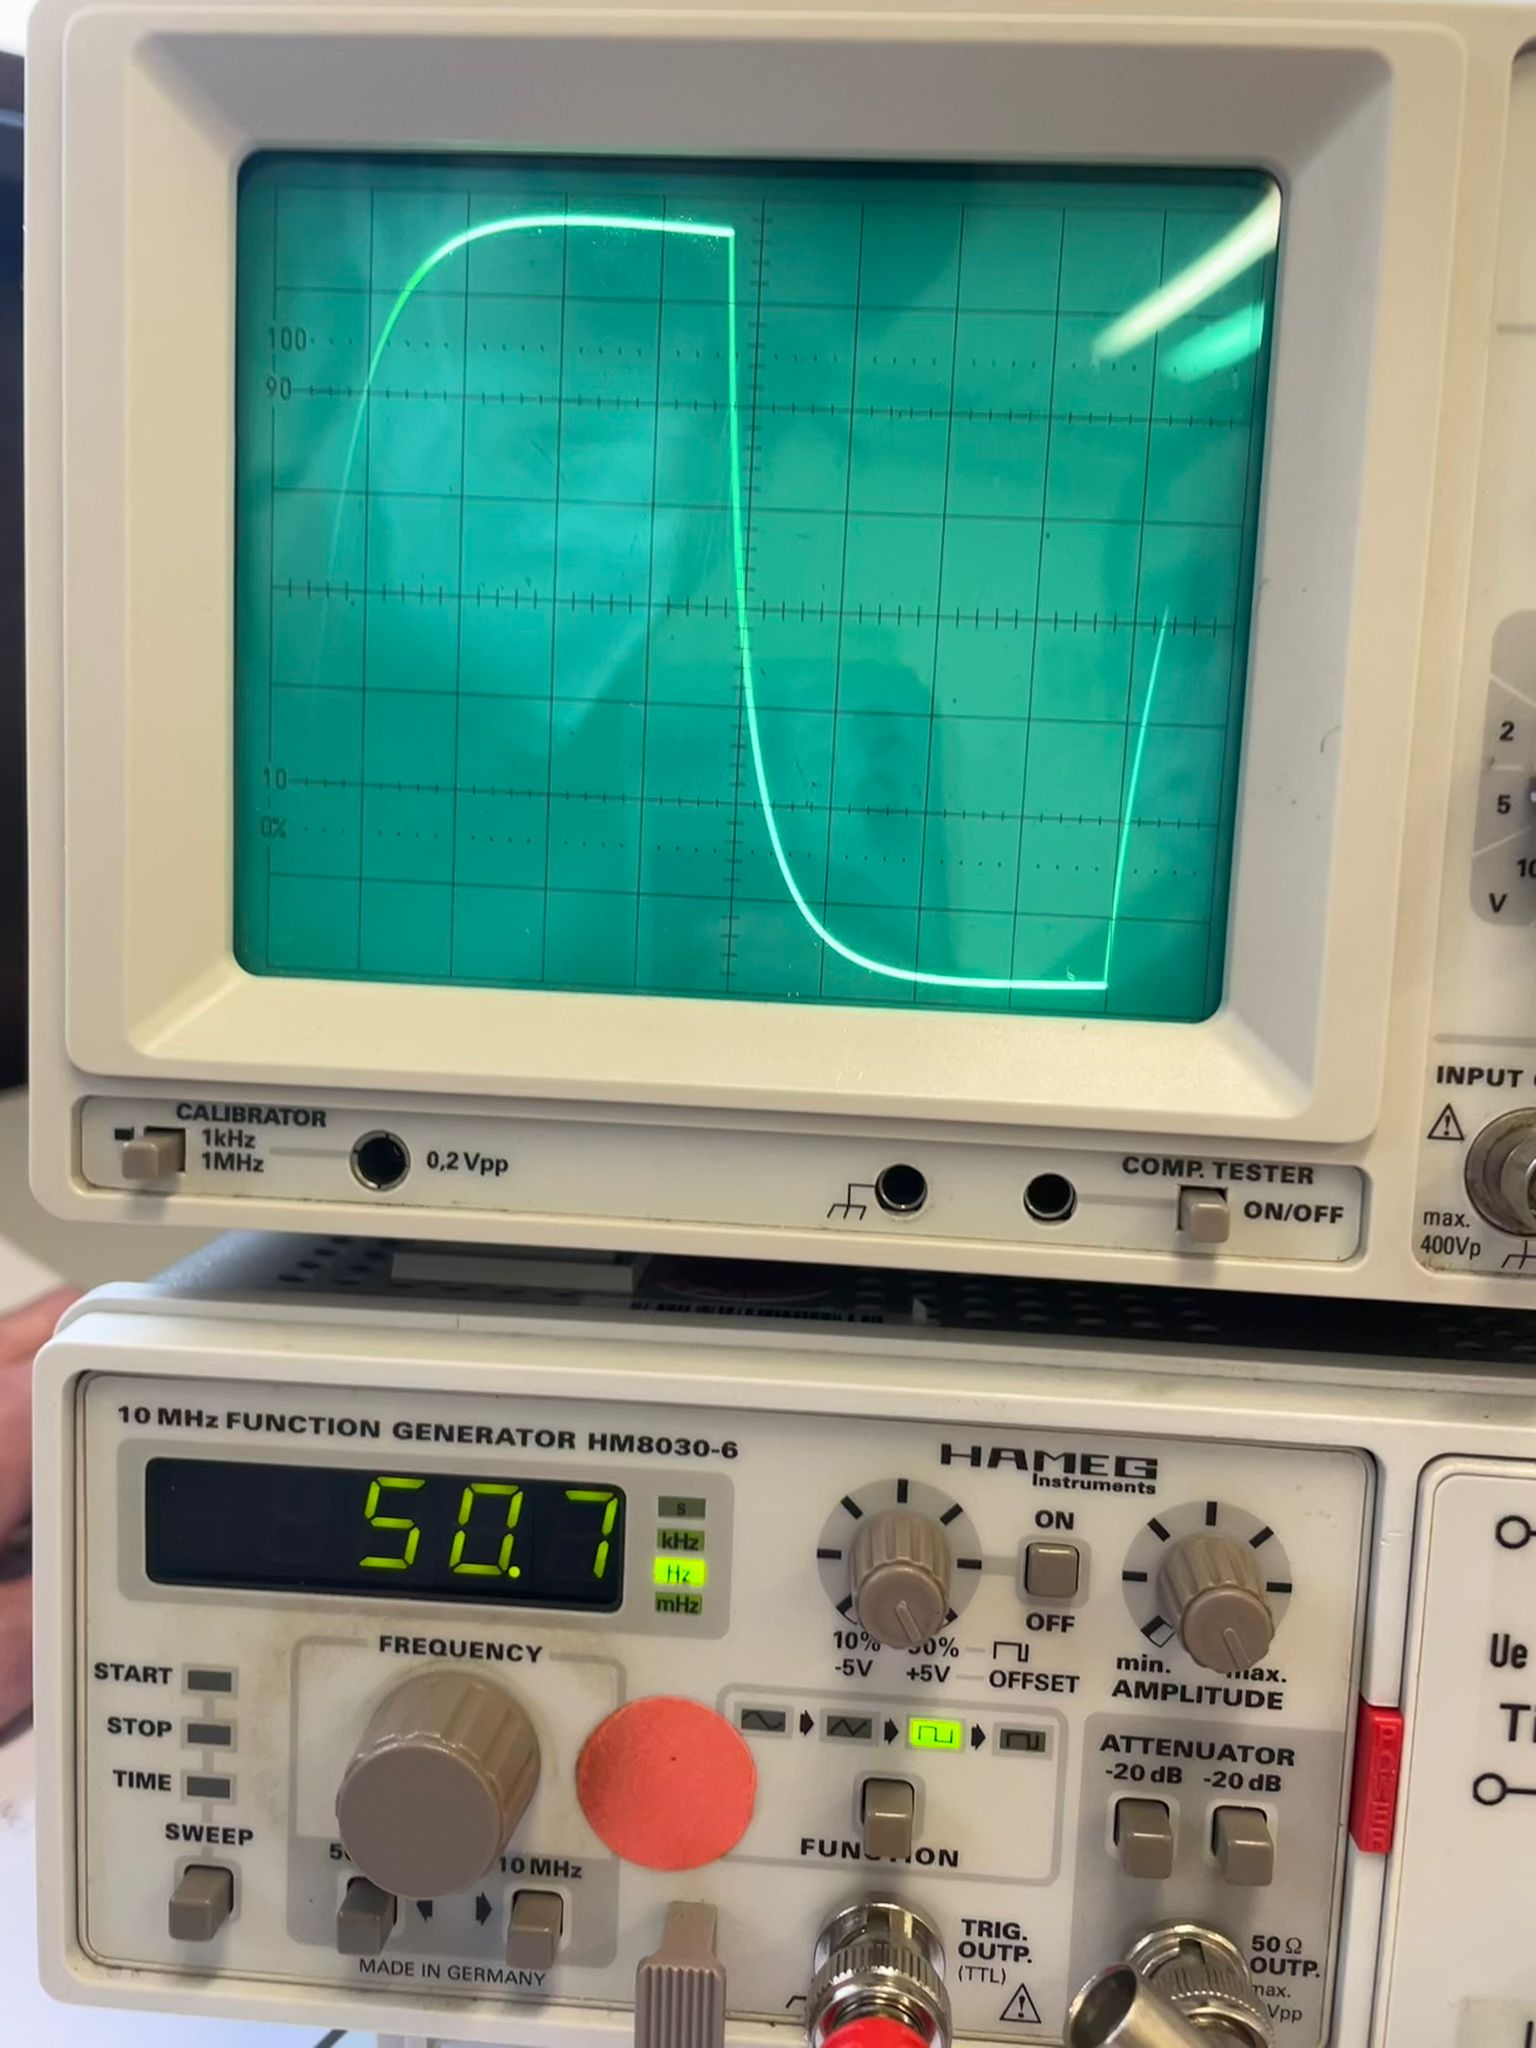
\includegraphics[scale=0.1]{content/entladung.png}
  \caption{Der Entladungsprozess des Kondensators.}
  \label{abb:Entladung}
\end{figure}

\begin{table}[H]
    \centering
    \caption{Eine Tabelle mit den aufgenommenen Messdaten aus \autoref{abb:Entladung} des Entladungsprozesses des Kondensators.}
    \label{tab:DatenEntladung}
    \begin{tabular}{
        S[table-format=1.1]
        S[table-format=1.2]
        S[table-format=-1.3]
        @{\hspace*{3em}\hspace*{\tabcolsep}}
        S[table-format=1.1]
        S[table-format=1.2]
        S[table-format=-1.3]
      }
        \toprule
        {$U_c \mathbin{/} \unit{\volt}$} &
        {$t \mathbin{/} \unit{\milli\second}$} &
        {$\ln(\frac{U_c}{U_0})$} &
        {$U_c \mathbin{/} \unit{\volt}$} &
        {$t \mathbin{/} \unit{\milli\second}$} &
        {$\ln(\frac{U_c}{U_0})$} \\
        \midrule
        3.4 & 0.04 & -0.057 & 1.6 & 0.30  & -0.811 \\
        3.2 & 0.08 & -0.118 & 1.4 & 0.34 & -0.944 \\
        3.0   & 0.09 & -0.182 & 1.2 & 0.48 & -1.099 \\
        2.8 & 0.10  & -0.251 & 1.0   & 0.53 & -1.281 \\
        2.6 & 0.13 & -0.325 & 0.8 & 0.62 & -1.504 \\
        2.4 & 0.16 & -0.405 & 0.6 & 0.73 & -1.792 \\
        2.2 & 0.19 & -0.492 & 0.4 & 0.90  & -2.197 \\
        2.0   & 0.24 & -0.588 & 0.2 & 1.10  & -2.890 \\
        1.8 & 0.28 & -0.693 & 0.1 & 1.40  & -3.584 \\
        \bottomrule
    \end{tabular}
\end{table}

Es wurden aus \autoref{abb:Entladung} die Werte in \autoref{tab:DatenEntladung} entnommen und nach Gleichung \eqref{RelQ} folgt 
für die lineare Regression:
\begin{equation}
  \label{eqn:linRegress}
    \ln\left(\frac{U_c}{U_0}\right)=-\frac{1}{RC}\cdot t + b.
\end{equation}
Woraus die Zeitkonstante $RC$ bestimmt wird.
Für die berechnung der Parameter a und b bei der linearen Regression für $y = ax + b$ gilt:
\begin{align*}
  \hat{a} &= \frac{\bar{xy}-\bar{x}\bar{y}}{\bar{x^2}-\bar{x}^2}\\
  \hat{b} &= \bar{y} - \hat{a}\bar{x}
\end{align*}
\begin{figure}[H]
  \centering
  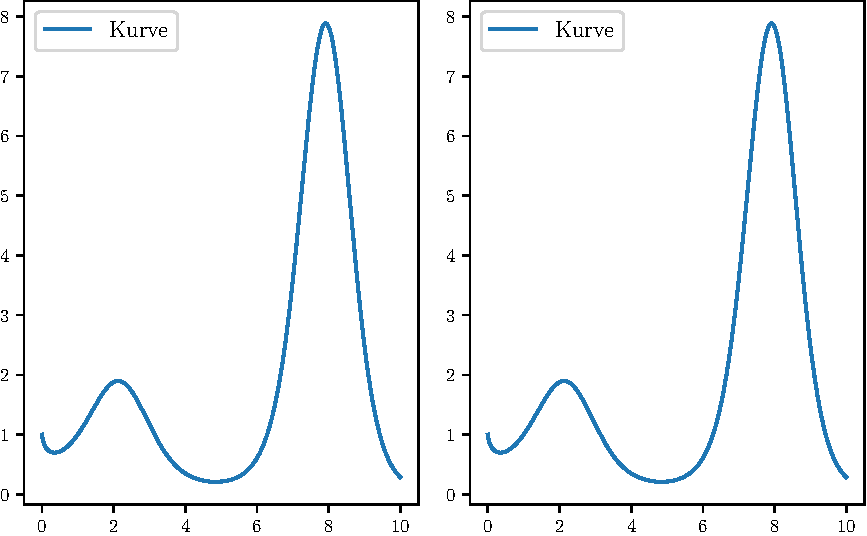
\includegraphics{plot.pdf}
  \caption{Lineare Regression nach \eqref{eqn:linRegress} und Messdaten aus \autoref{tab:DatenEntladung} zur Bestimmung der Zeitkonstante RC über den Entladungsprozesses des Kondensators.}
  \label{fig:plot}
\end{figure}

Es ergibt sich aus der linearen Regression in \autoref{fig:plot}:
\begin{align*}
  RC &= (0.3900\pm 0.0006)\unit{\milli\second}\\
  b &= 0.0309\pm 0.0214.\\
\end{align*}
%(-2564.035208002769, 37.56001783858995, 0.03087285853896417, 0.02142147040602549)
\begin{table}[H]
  \centering
  \caption{Die Tabelle mit den Wertepaaren für die Bestimmung von $RC$ über die Relativamplitude.}
  \label{tab:DatenB}
  \begin{tabular}{
      S[table-format=2.4]
      S[table-format=1.2]
    }
      \toprule
      {$f \mathbin{/} \unit{\kilo\hertz}$} &
      {$\frac{U_c}{U_0} \mathbin{/} \unit{\volt}$} \\
      \midrule
      0.1100  & 2.083 \\
      0.1890  & 1.667 \\
      0.2500  & 1.389 \\
      0.2995 & 1.111 \\
      0.4008 & 0.944 \\
      0.5140  & 0.611 \\
      0.9980  & 0.444 \\
      2.0510  & 0.222 \\
      3.1200   & 0.167 \\
      5.1700   & 0.069 \\
      9.0800   & 0.056 \\
      22.3400  & 0.022 \\
      30.3700  & 0.017 \\
      35.1500  & 0.014 \\
      40.0900  & 0.011 \\
      42.3300  & 0.011 \\
      44.0500  & 0.011 \\
      46.1600  & 0.011 \\
      48.3200  & 0.011 \\
      51.2400  & 0.008 \\
      \bottomrule
  \end{tabular}
\end{table}

Anschließend wurde die Zeitkonstante $RC$ mit den Wertepaaren der Relativamplitude $\frac{U_c}{U_0}$ und der Generatorfrequenz $f$
aus \autoref{tab:DatenB} mithilfe der folgenden Ausgleichsrechnung nach \eqref{eqn:bezAU} bestimmt:
\begin{equation}
  \label{eqn:Ausgleichsrechnung1}
  \frac{U_c}{U_0} = \frac{1}{\sqrt{1+a^2(2\pi f)^2}}
\end{equation}
Wobei bei dieser Ausgleichsrechnung die Zeitkonstante $RC = a$ ist und in \autoref{fig:plot2} dargestellt ist.
\begin{figure}[H]
  \centering
  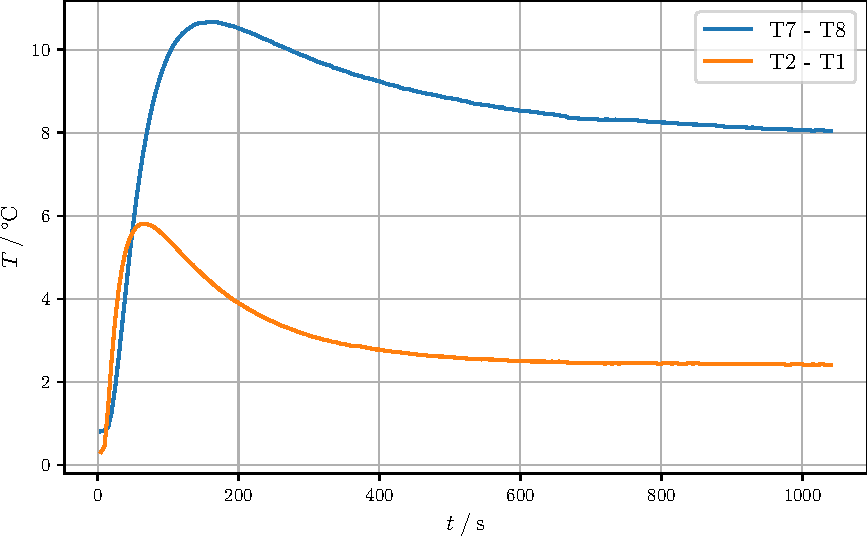
\includegraphics{plot2.pdf}
  \caption{Hier sind die Wertepaare aus \autoref{tab:DatenB} die Ausgleichsrechnung nach \eqref{eqn:Ausgleichsrechnung1} und die Originalfunktion nach \eqref{eqn:bezAU} mit dem berechneten $RC$ in einem halblogarithmischen Diagramm aufgetragen.}
  \label{fig:plot2}
\end{figure}

Es ergibt sich der Parameter a und b der Ausgleichsrechnung zu:
\begin{align*}
  a &= (-0.7531\pm 0.0363) \unit{\milli\second}\\
  RC &= (0.7531\pm 0.0363) \unit{\milli\second}
\end{align*}

\begin{table}[H]
  \centering
  \caption{Eine Tabelle mit den Wertepaaren für Teilaufgabe c) mit den aus den Messwerten von a und b aus \autoref{tab:DatenAbgelesen} mit Formel $\frac{a}{b}\cdot 2\pi = \varphi$ berechneten $\varphi$.}
  \label{tab:DatenC}
  \begin{tabular}{
      S[table-format=2.4]
      S[table-format=1.4]
    }
      \toprule
      {$f \mathbin{/} \unit{\kilo\hertz}$} &
      {$\symup{\varphi} \mathbin{/} \unit{\radian}$}\\
      \midrule
      0.1100  & 0.6283 \\
      0.1890  & 0.8568 \\
      0.2500  & 1.1088 \\
      0.2995 & 1.1220 \\
      0.4008 & 1.2566 \\
      0.5140  & 1.1968 \\
      0.9980  & 1.4280 \\
      2.0510  & 1.2566 \\
      3.1200   & 1.7952 \\
      5.1700   & 1.5708 \\
      9.0800   & 1.5708 \\
      22.3400  & 1.2566 \\
      30.3700  & 1.7952 \\
      35.1500  & 2.0944 \\
      40.0900  & 2.0944 \\
      42.3300  & 1.2566 \\
      44.0500  & 1.2566 \\
      46.1600  & 1.2566 \\
      48.3200  & 1.2566 \\
      51.2400  & 1.4784 \\
      \bottomrule
  \end{tabular}
\end{table}

Die dritte Methode, die Zeitkonstante $RC$ zu bestimmen, basiert auf einer Ausgleichsrechung zu den Wertepaaren der Phasenverschiebung $\varphi$ 
und der Generatorfrequenz $f$ aus \autoref{tab:DatenC}.
Die Ausgleichsrechnung ergibt sich in diesem Fall nach \eqref{PhiArctan} zu:
\begin{equation}
  \label{eqn:Ausgleichsrechnung2}
  \symup{\varphi} = a\cdot\arctan(b\cdot t).
\end{equation}
Wobei hier die Zeitkonstante $RC = b$ ist.
\begin{figure}[H]
  \centering
  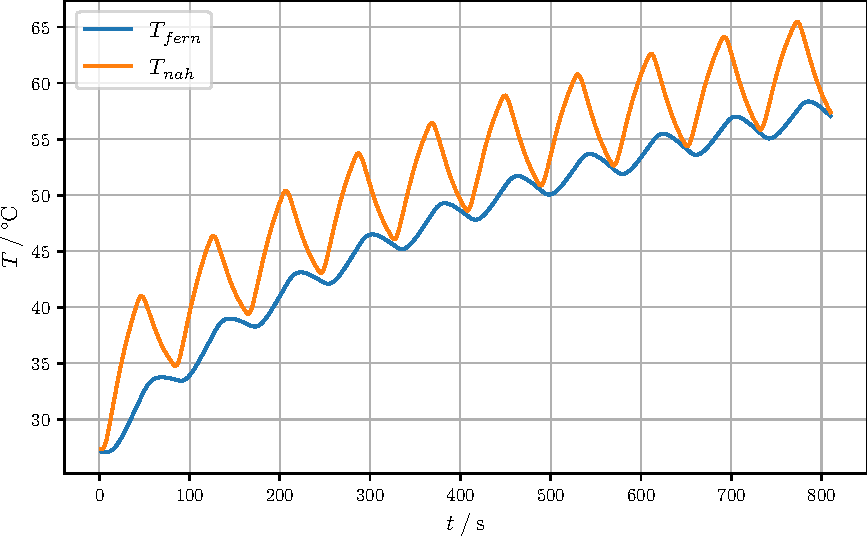
\includegraphics{plot3.pdf}
  \caption{Hier sind die Wertepaare aus \autoref{tab:DatenC}, die Ausgleichsrechnung nach \eqref{eqn:Ausgleichsrechnung2} und die Originalfunktion nach \eqref{PhiArctan} mit eingesetztem $RC$ in einem halblogarithmischem Diagramm aufgetragen.}
  \label{fig:plot3}
\end{figure}
Bei dieser Ausgleichsrechnung ergeben sich die Parameter a und b zu:
\begin{align*}
  a &=0.9862\pm 0.0464 \\
  b &=(6.9641\pm 2.0824) \unit{\milli\second} = RC \\
\end{align*}

Die Abhängigkeit der Relativamplitude $\frac{U_c}{U_0}$ von der Phase $\varphi$ ergibt sich zu:
\begin{equation*}
  \frac{U_c}{U_0} = \cos\left(\varphi\right).
\end{equation*}

\begin{table}[H]
  \centering
  \caption{Die Wertepaare für den Polarplot}
  \label{tab:DatenD}
  \begin{tabular}{
      S[table-format=1.3]
      S[table-format=1.4]
    }
      \toprule
      {$\frac{U_c}{U_0} \mathbin{/} \unit{\volt}$} &
      {$\symup{\varphi} \mathbin{/} \unit{\radian}$}\\
      \midrule
      2.083 & 0.6283 \\
      1.667 & 0.8568 \\
      1.389 & 1.1088 \\
      1.111 & 1.1220 \\
      0.944 & 1.2566 \\
      0.611 & 1.1968 \\
      0.444 & 1.4280 \\
      0.222 & 1.2566 \\
      0.167 & 1.7952 \\
      0.069 & 1.5708 \\
      0.056 & 1.5708 \\
      0.022 & 1.2566 \\
      0.017 & 1.7952 \\
      0.014 & 2.0944 \\
      0.011 & 2.0944 \\
      0.011 & 1.2566 \\
      0.011 & 1.2566 \\
      0.011 & 1.2566 \\
      0.011 & 1.2566 \\
      0.008 & 1.4784 \\
      \bottomrule
  \end{tabular}
\end{table}

\begin{figure}[H]
  \centering
  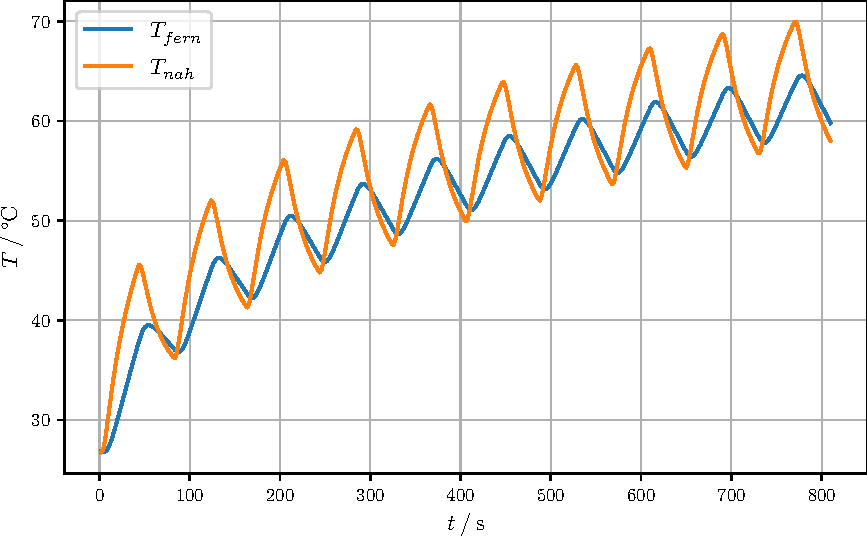
\includegraphics{plot4.pdf}
  \caption{Hier wurde die erwähnte Abhängigkeit der Relativamplitude von der Phase, sowie einige Wertepaare aus \autoref{tab:DatenD} in ein Polardiagramm eingetragen.}
  \label{fig:plot4}
\end{figure}

\begin{figure}
  \centering
  \textbf{Integration verschiedener Generatorspannungen bei einer Frequenz $\symbf{f = 4726\unit{\hertz}}$}\par\medskip
  \begin{subfigure}{0.48\textwidth}
    \centering
    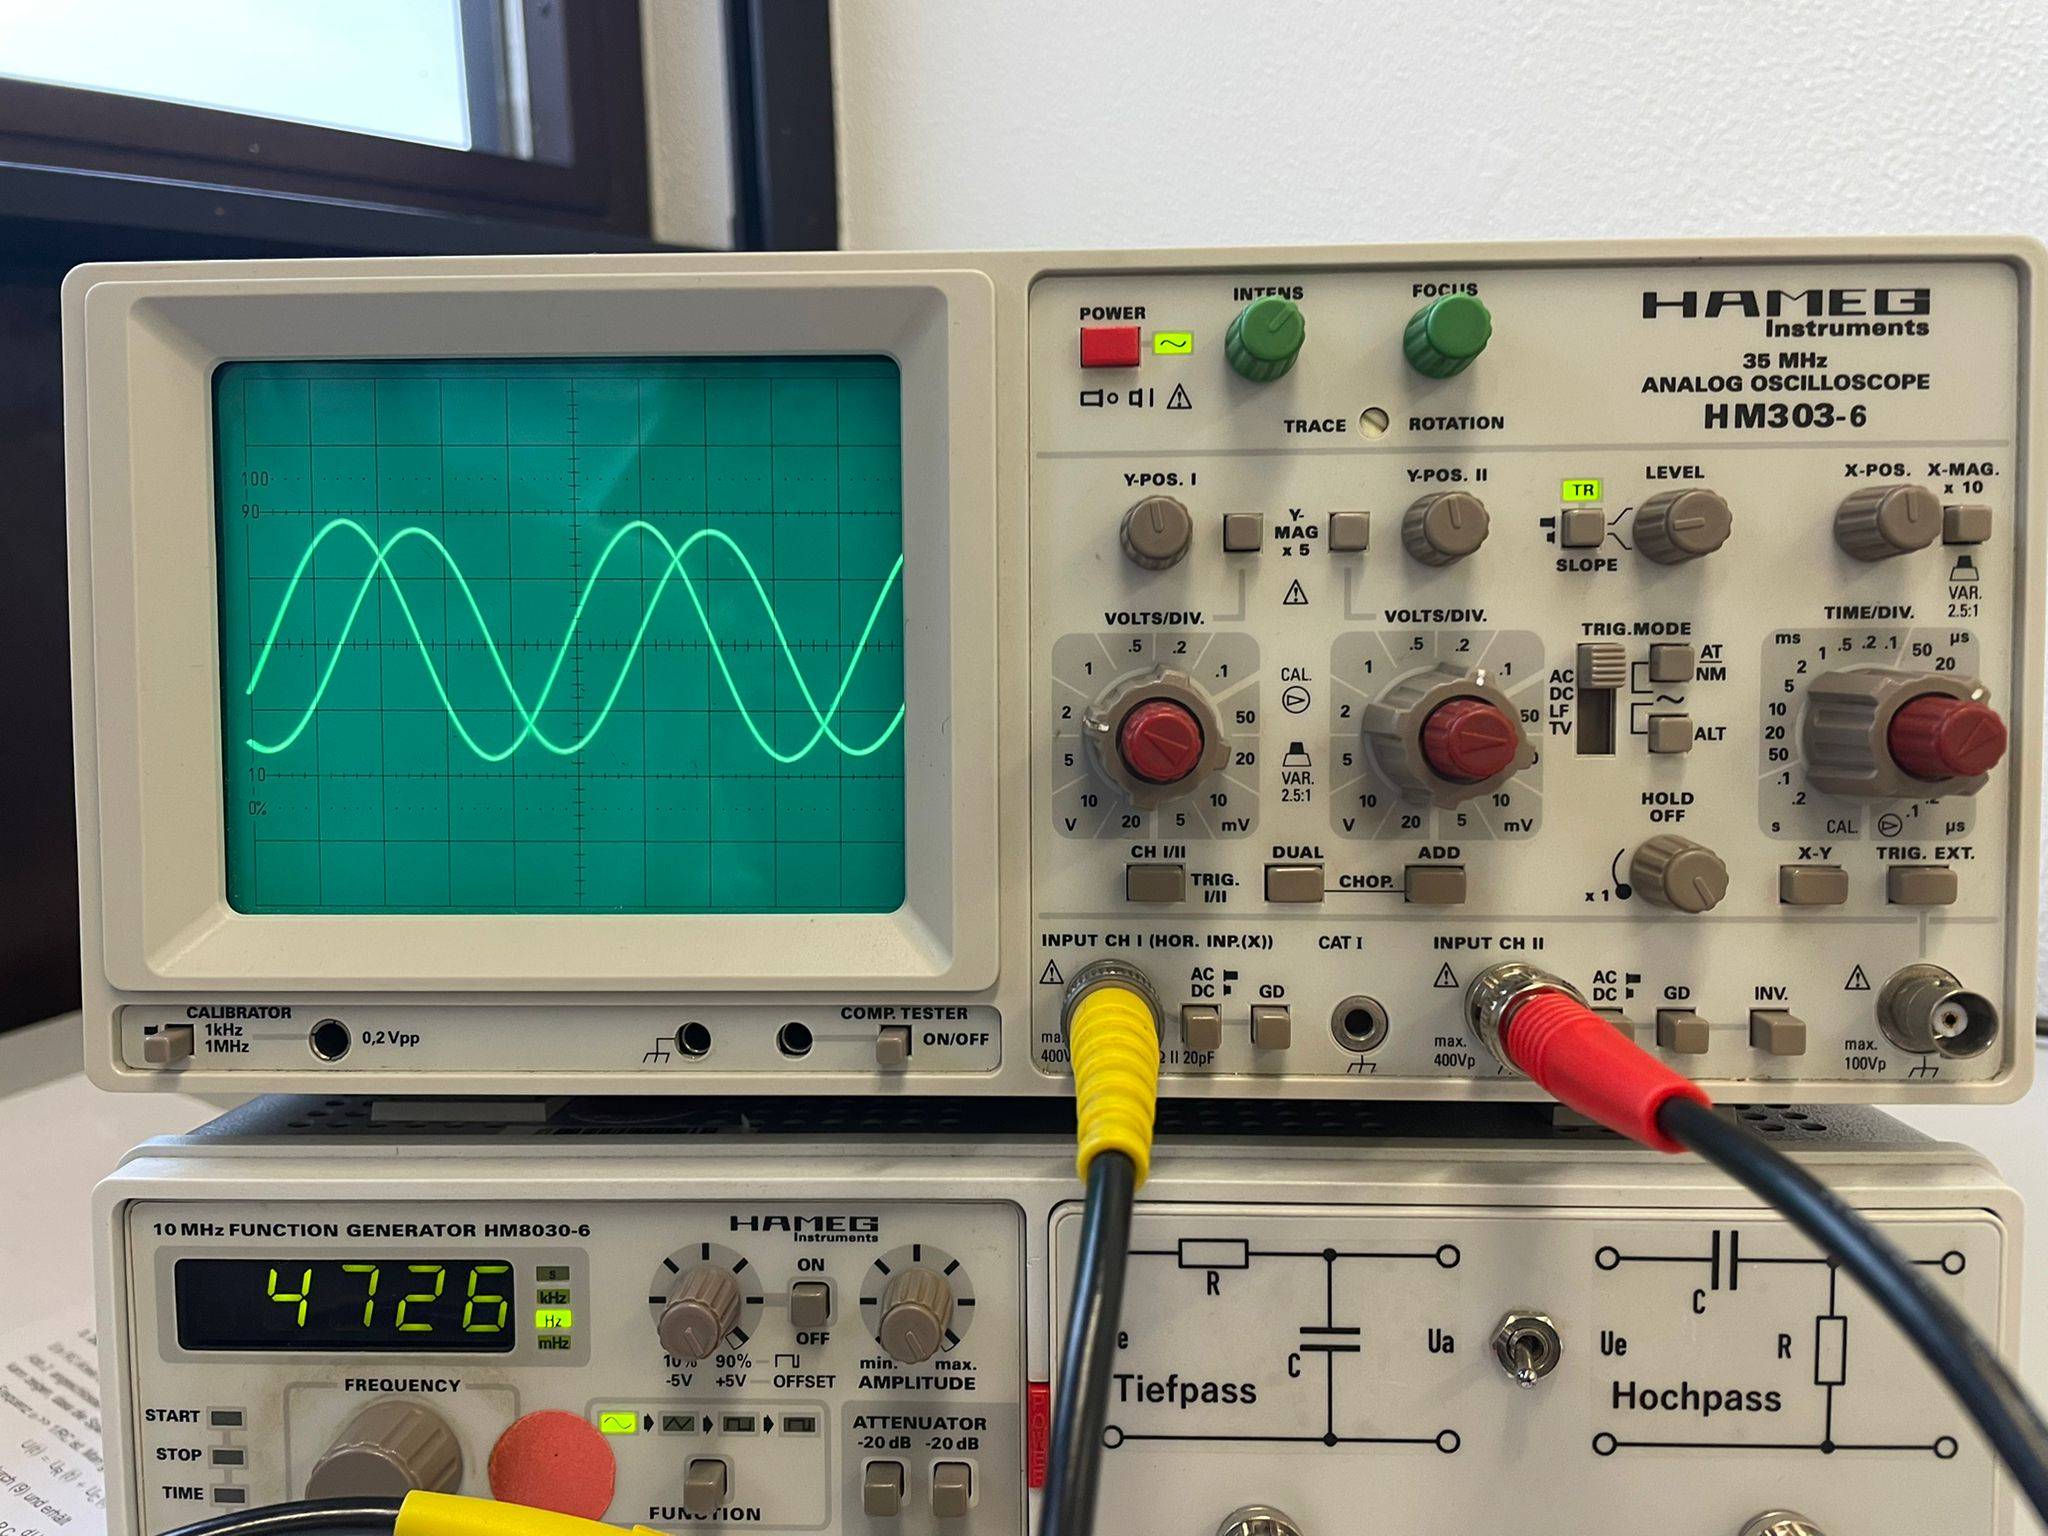
\includegraphics[scale=0.1]{content/sinInt.png}
    \caption{sin}
  \end{subfigure}
  \hfill
  \begin{subfigure}{0.48\textwidth}
    \centering
    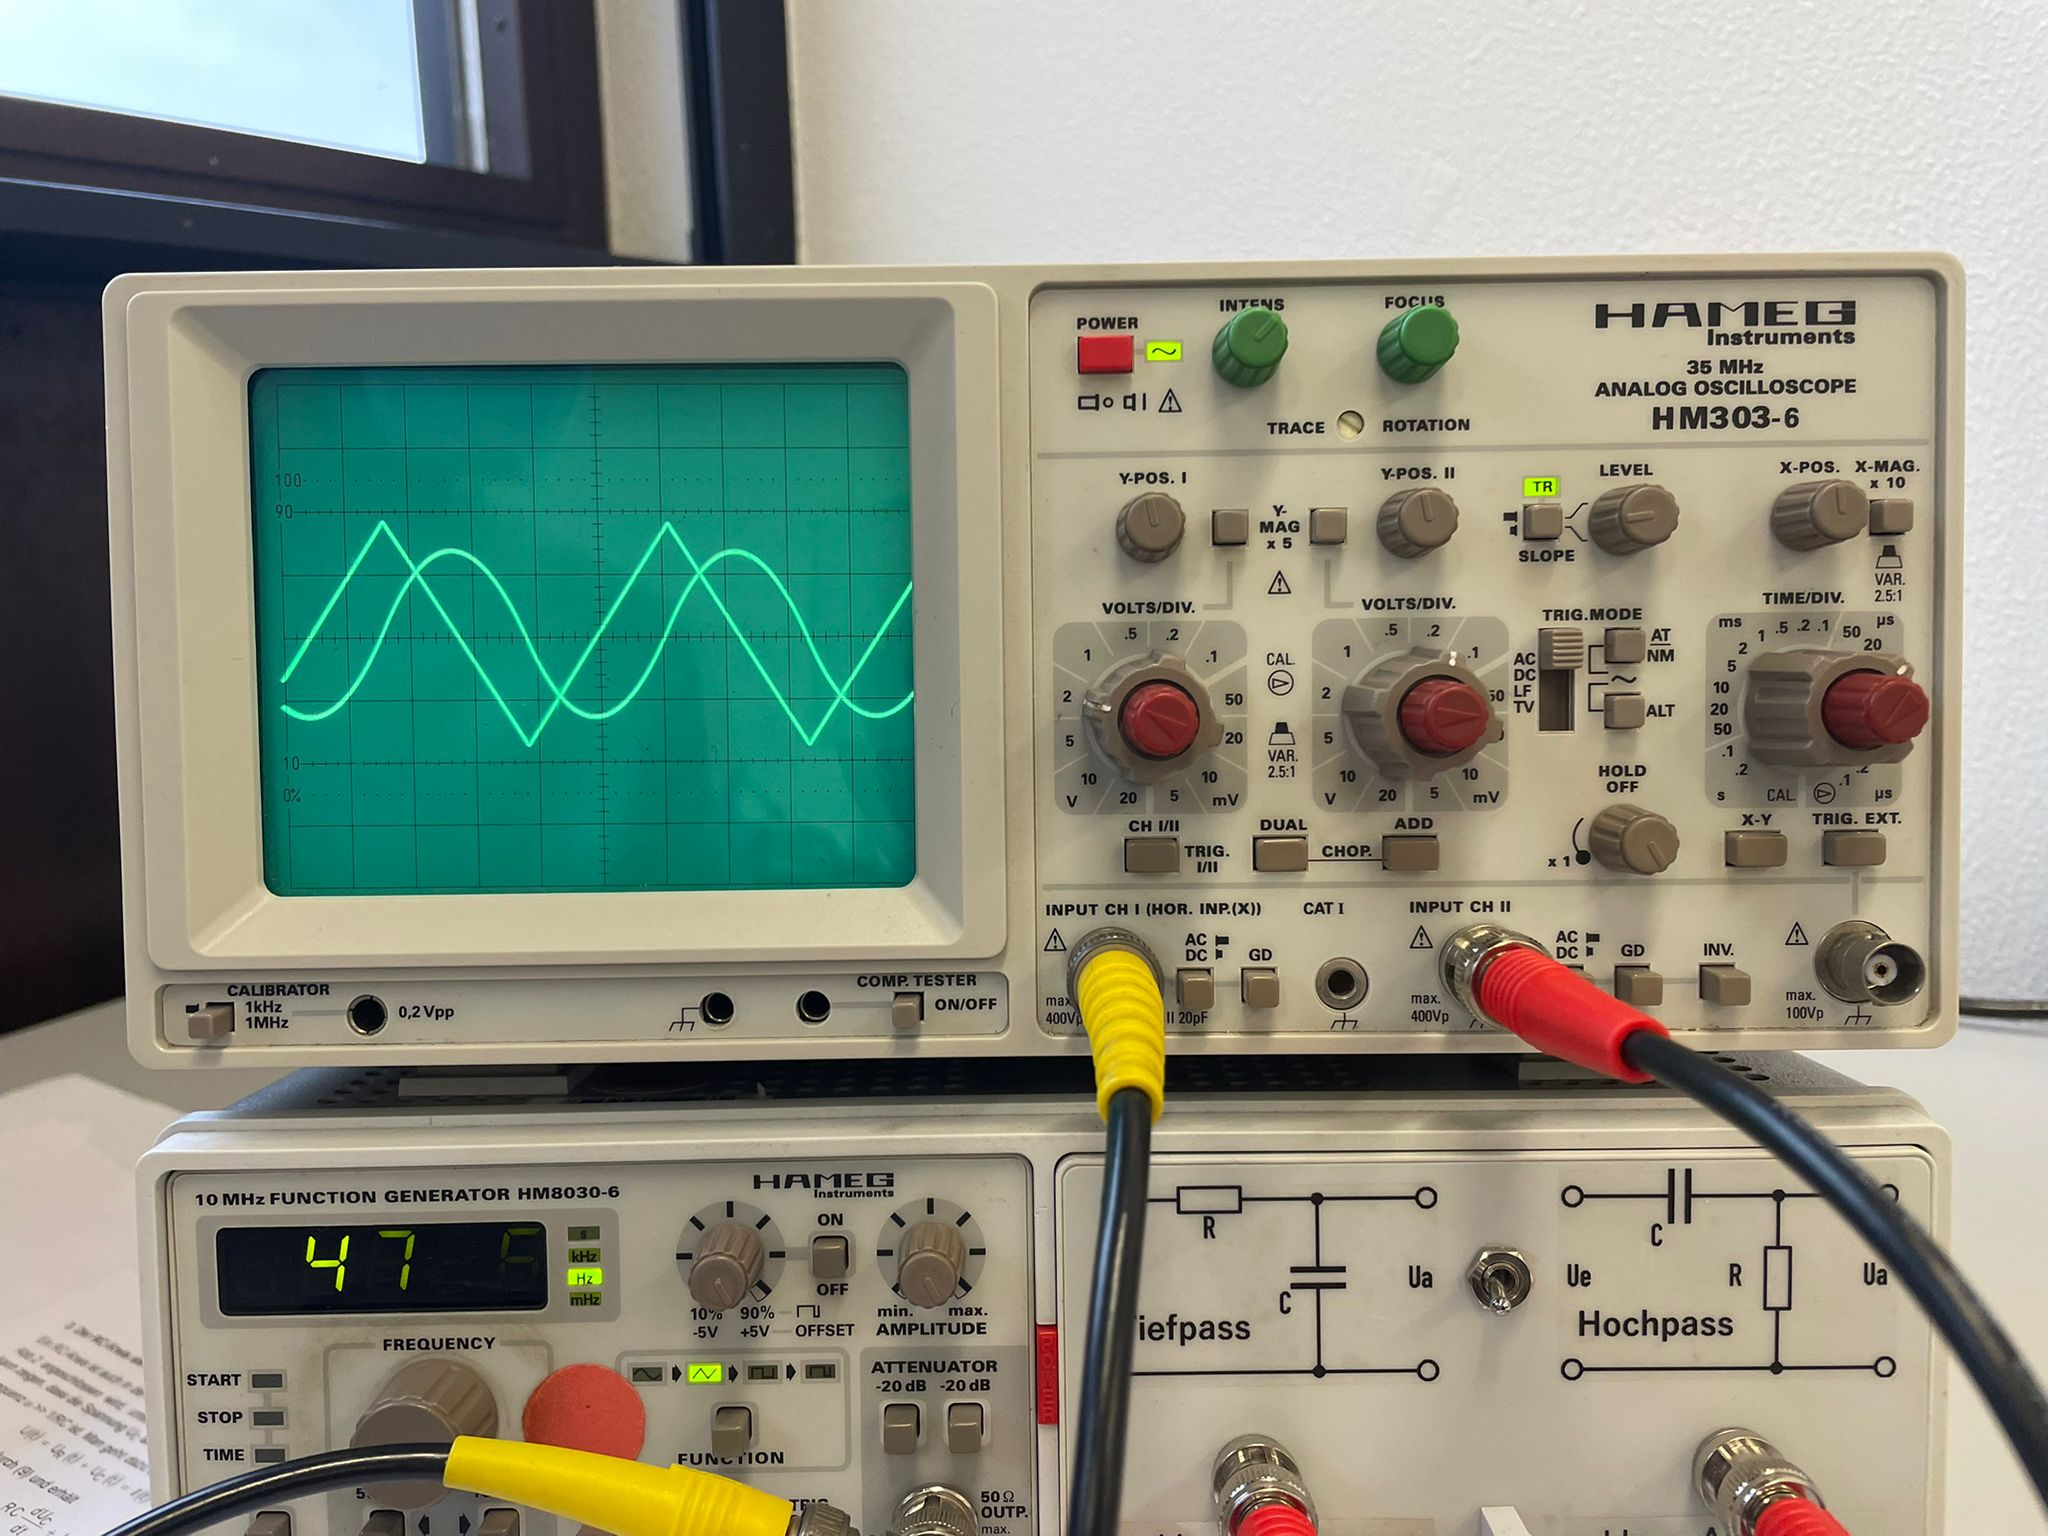
\includegraphics[scale=0.1]{content/saegInt.png}
    \caption{Sägezahn}
  \end{subfigure}
  \caption{}
\end{figure}

\begin{figure}
  \centering
  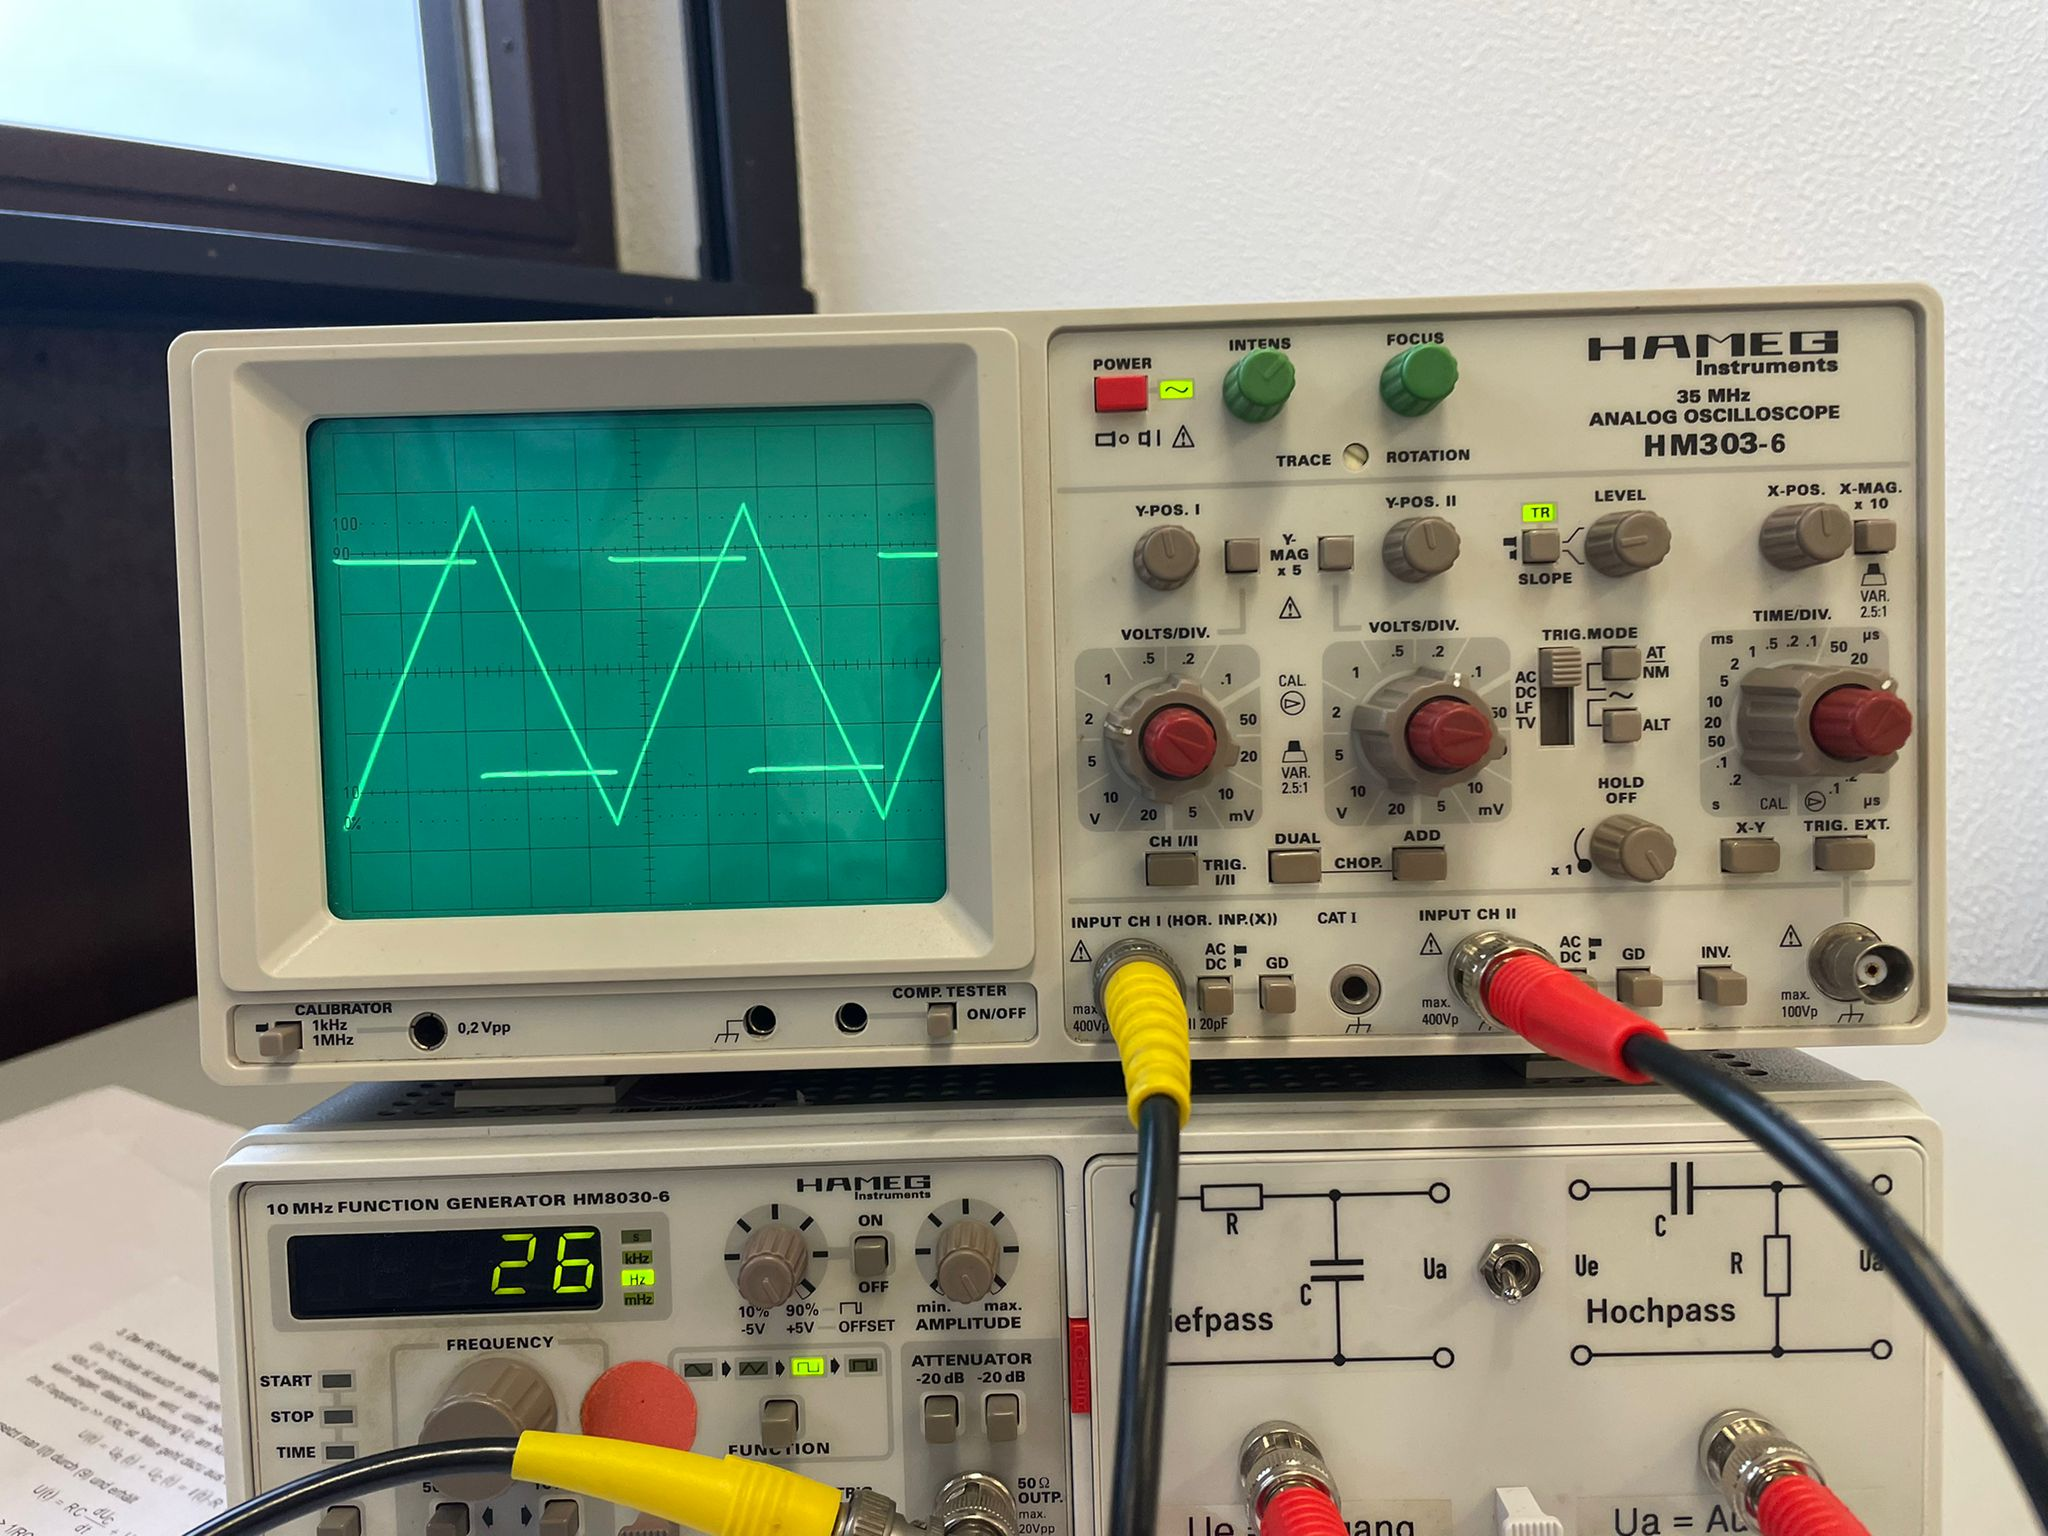
\includegraphics[scale=0.1]{content/rechteckInt.png}
  \caption{Rechteck}
\end{figure}
